\section{機器監視サービスの構成}
%(どのような要素で構成されているのか,また,それぞれの役割は何なのか)
%1.1全体構成(どのような要素で構成され,また,それぞれの役割について簡潔に述べる)
第3章にて述べた要件に基づき,システムを構築した.
システムは,エージェントプログラム,機器状態データベース,機器情報データベース,エージェントプログラム用インターフェースプログラム,Webアプリケーションサーバ,Webアプリケーションから成り立っている.
エージェントプログラムとエージェントプログラム用インターフェース,WebアプリケーションサーバとWebアプリケーションは,インターネットを介して通信しあう.
図\ref{fig:blockdiagram}は、システムのブロック図である。
\medskip

\begin{figure}[htbp]
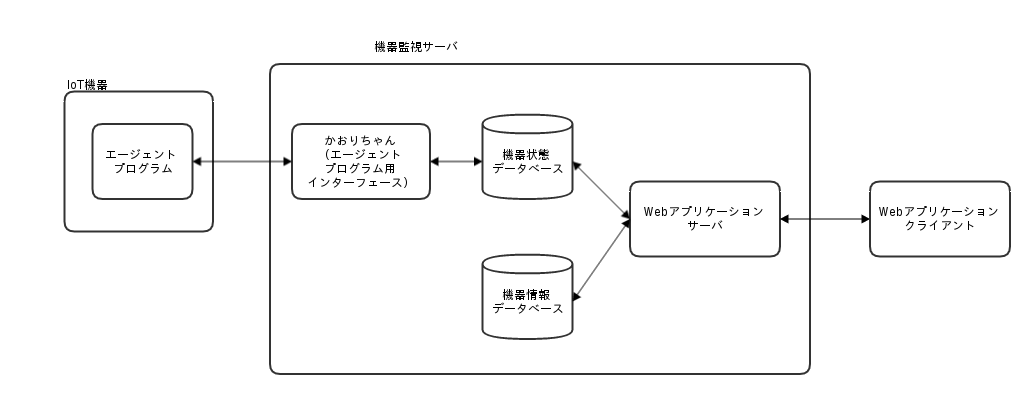
\includegraphics[width=16cm]{images/blockdiagram2.png}
\caption{システムのブロック図}
\label{fig:blockdiagram}
\end{figure}

エージェントプログラムは,IoT機器上で動作するプログラムである.
定期的に自身の状態を状態蓄積システムへ送信する役割を果たす.
定期的かつ自発的に状態を送信することで,ネットワーク環境によらない機器の監視を可能にした.
IoT機器として頻繁に使用されるRaspberryPiを想定し作成した。
「かおりちゃん」とは,エージェントプログラム用インターフェースである.
各IoT機器上で動くエージェントプログラムから送られてきた状態を,時刻と共に機器状態データベースへ書き込む役割を果たすプログラムで,機器監視サーバー上で動作する.
機器状態データベースとは,機器の状態を時系列に沿って蓄積するデータベースである.
機器監視サーバー上で動作する.
機器情報データベースとは,機器IDや,機器名,ユーザー名を記録するデータベースである.
機器監視サーバー上で動作する.
\medskip

Webアプリケーションサーバーは,WebページやWebアプリケーション自体を配信する.
ユーザーが利用するブラウザからの要求に答え,現在の機器の状態や,機器名等を返答する.
\medskip

Webアプリケーションとは,ブラウザ上で動作するプログラムである.
ユーザーからの入力を受け付け、ユーザーへ表示する他、必要な機能を問い合わせる。
\medskip

これら各要素が連携することで,機器の監視を実現している。

\subsection{エージェントプログラム}
%(エージェントプログラムとは何なのか)
エージェントプログラムとは,IoT機器上にインストールされるプログラムである.
エージェントプログラムの役割は,定期的に送信失敗回数を「かおりちゃん」へ報告することである.
送信失敗回数とは,ネットワークの不具合等により,機器監視サーバーへ送信されなかった報告の数である.
自発的に状態を報告するため,IoT機器にプライベートアドレスが付与されていても,状態を検知することができる.
また,HTTPを用いるため,間のネットワークにてブロックされることがない.

\subsection{エージェントプログラム用インターフェース}
エージェントプログラム用インターフェースとは,サーバー上で動くプログラムである.名前を「かおりちゃん」とした。
エージェントプログラム用インターフェースの役割は,エージェントプログラムから送信されたメッセージを受け取り,現在の時刻と正常である旨を機器状態データベースへ書き込む.
また,エージェントプログラムから送られた送信失敗回数から,IoT機器がインターネットから切断された時刻を逆算し,機器状態データベースへ書き込む事も行う.

\subsection{機器状態データベース}
%(とは何なのか)
機器状態データベースとは,サーバ上で動作するデータベースである.
各IoT機器の状態を時刻とともに記録する.
機器状態監視システムの中心にあるデータベースである.

\subsection{機器情報データベース}
機器情報データベースとは,サーバー上で動作するデータベースである.
各IoT機器の機器ID,機器名,機器詳細情報,ユーザーのメールアドレスとパスワードを記録する.

\subsection{Webアプリケーションサーバ}
Webアプリケーションサーバとは,サーバ上で動作するプログラムである.
WebアプリケーションやWebページの配信,Webアプリケーションからの要求の処理などを行う.
必要に応じて,機器状態データベースと機器情報データベースへアクセスを行う.
次に,Webアプリケーションとのインターフェースを挙げ,それぞれについて説明する.
\subsubsection{ログインAPI}
Webアプリケーションから,メールアドレスとパスワードを受け取り,	機器情報データベースのユーザーテーブルと照合する.
照合した結果,ユーザー名とパスワードが合致したユーザーが存在すれば,HTTPクッキーにセッションキーをセットし,機器状態一覧ページへのリダイレクトを返す.
合致したユーザーが存在しなかった場合,エラーメッセージを返す.
\subsubsection{ログアウトAPI}
Webアプリケーションに,HTTPクッキーから該当のセッションキーを削除するよう要求する.
\subsubsection{機器情報・機器状態取得API}
ログインチェックを行った後,機器情報データベースと機器状態データベースより,全IoT機器の機器情報と機器状態を返す.
\subsubsection{機器ID生成API}
ログインチェックを行った後,機器情報データベースに存在しない,ランダムな機器IDを返す.
\subsubsection{機器ID重複チェックAPI}
ログインチェックを行った後.Webアプリケーションから機器IDを受け取る.
機器情報データベースに該当の機器IDが存在するかしないかを返す.
\subsubsection{機器作成API}
ログインチェックを行った後,Webアプリケーションから,機器ID,機器名,機器の詳細と,機器の作成なのか編集なのかの指示を受け取る.
機器の作成であった場合,
機器IDに重複が無いことを確認したうえで,機器情報データベースに該当のエントリを作成・機器状態データベースにメジャーメントを作成する.
作成されたか,されなかったかを返す.
機器の編集であった場合,
機器情報データベースから,受け取った機器IDを持つものを探しだし,編集する.
編集できたか否かを返す.
\subsubsection{機器削除API}
ログインチェックを行った後,Webアプリケーションから,機器IDを受け取る.
機器情報データベースから,受け取った機器IDを持つものを削除する.
その後,機器状態データベースから,メジャーメントを削除する.
削除されたか否かを返す.
\subsubsection{過去の機器状態取得API}
ログインチェックを行った後,機器状態データベースから,全てのIoT機器の過去の状態をまとめ,返す.

\subsection{Webアプリケーション}
Webアプリケーションとは,ユーザーのブラウザ上で動作するアプリケーションである.
ユーザーへグラフィカルインターフェースを提供する.
必要に応じて,Webアプリケーションサーバへ必要な情報を要求する.
Webアプリケーションは,3つのWebページから成り立っている.
以下に各ページとそれぞれの役割を述べる.
\begin{itemize}
	\item ログインページ\\
		正当なユーザーであることを確認するために,メールアドレスとパスワードの入力を求める.
		メールアドレスとパスワードは,Webアプリケーションサーバーへ送信される.
		図\ref{fig:ss_login}は、ログインページのスクリーンショットである。
		\begin{figure}[htbp]
		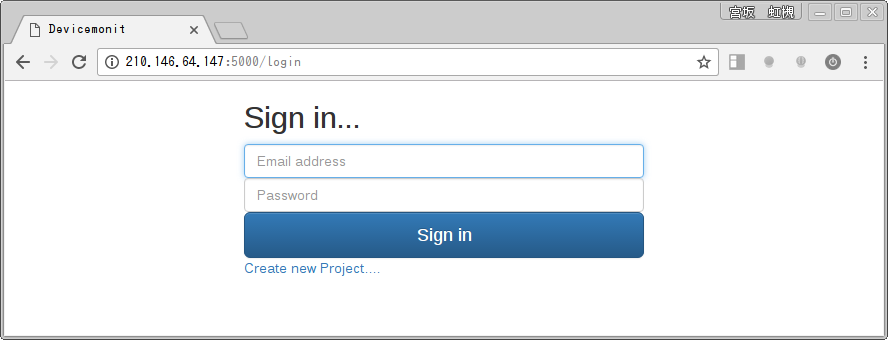
\includegraphics[width=16cm]{images/login.png}
		\caption{ログイン画面}
		\label{fig:ss_login}
		\end{figure}

	\item 機器状態一覧ページ\\
		機器状態を一覧して表示する他,機器の作成や,機器情報の編集,機器の削除等を行う事ができる.
		現在の機器の状態を取得するため,定期的にWebアプリケーションサーバと通信する.
		また,機器の作成や機器情報の編集,削除の為,Webアプリケーションサーバと通信する.

		図\ref{fig:ss_sum1}・図\ref{fig:ss_sum2}・図\ref{fig:more}はこのページのスクリーンジョットである。
		それぞれ、一覧表示・縮小一覧表示・詳細な情報の表示をしている。
		図\ref{fig:ss_add}・図\ref{fig:ss_mod}は、それぞれ、機器追加ダイアログ・機器情報編集ダイアログのスクリーンショットである。
		\begin{figure}[htbp]
		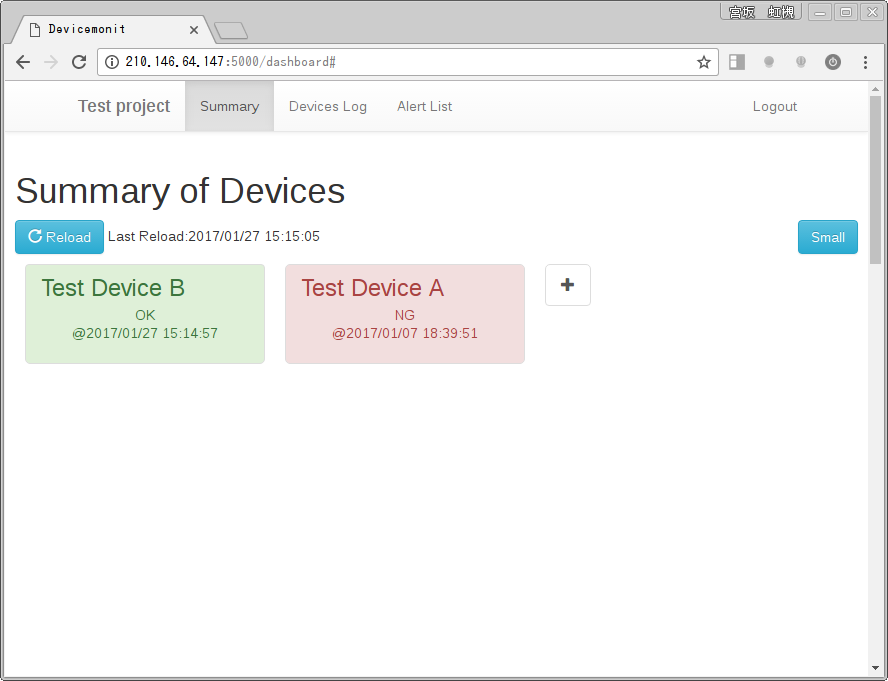
\includegraphics[width=16cm]{images/screenshot_summary1.png}
		\caption{機器状態一覧画面}
		\label{fig:ss_sum1}
		\end{figure}

		\begin{figure}[htbp]
		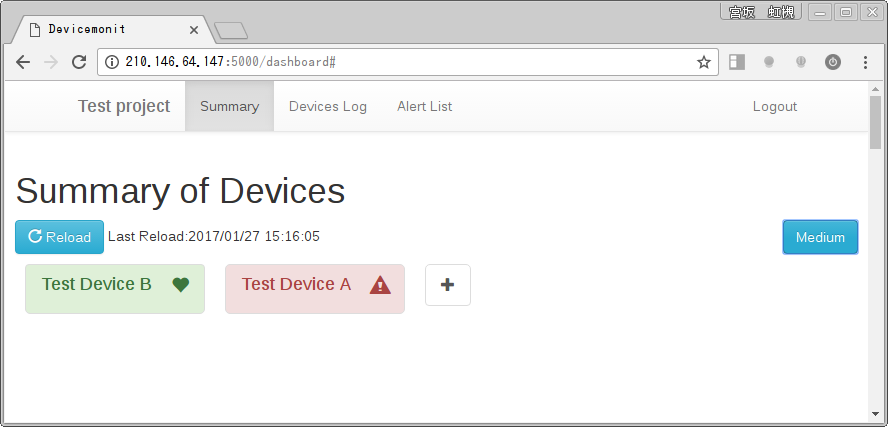
\includegraphics[width=16cm]{images/screenshot_summary2.png}
		\caption{機器状態一覧画面(小さく表示)}
		\label{fig:ss_sum2}
		\end{figure}

		\begin{figure}[htbp]
		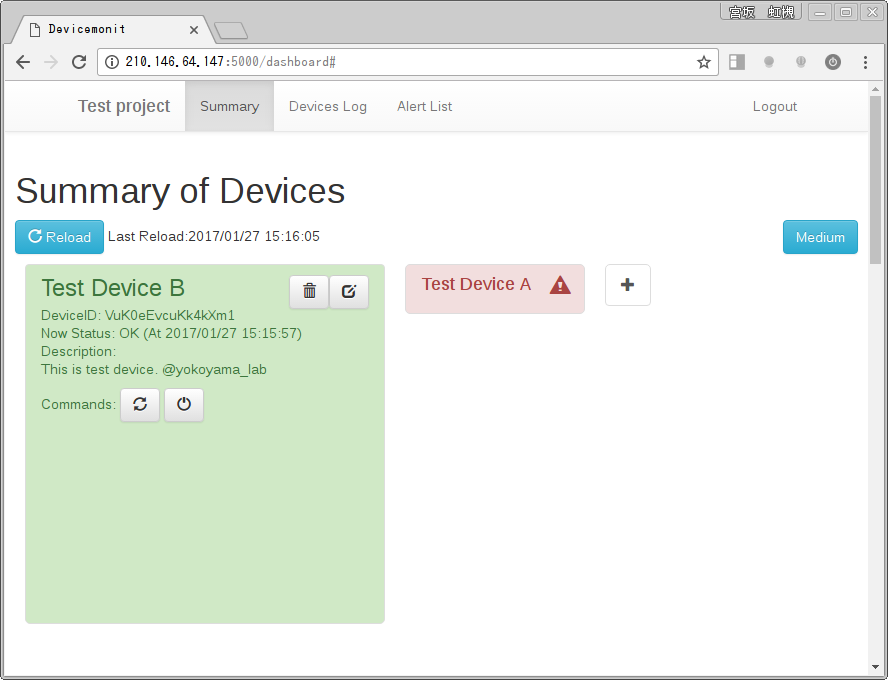
\includegraphics[width=16cm]{images/screenshot_more.png}
		\caption{機器状態詳細表示}
		\label{fig:ss_more}
		\end{figure}

		\begin{figure}[htbp]
		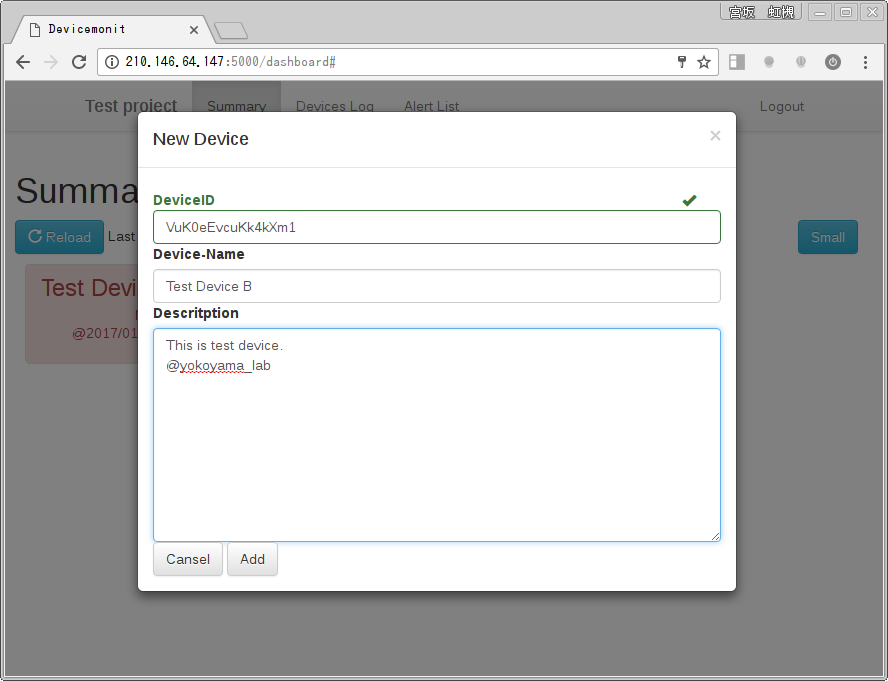
\includegraphics[width=16cm]{images/screenshot_add.png}
		\caption{機器追加ダイアログ}
		\label{fig:ss_add}
		\end{figure}

		\begin{figure}[htbp]
		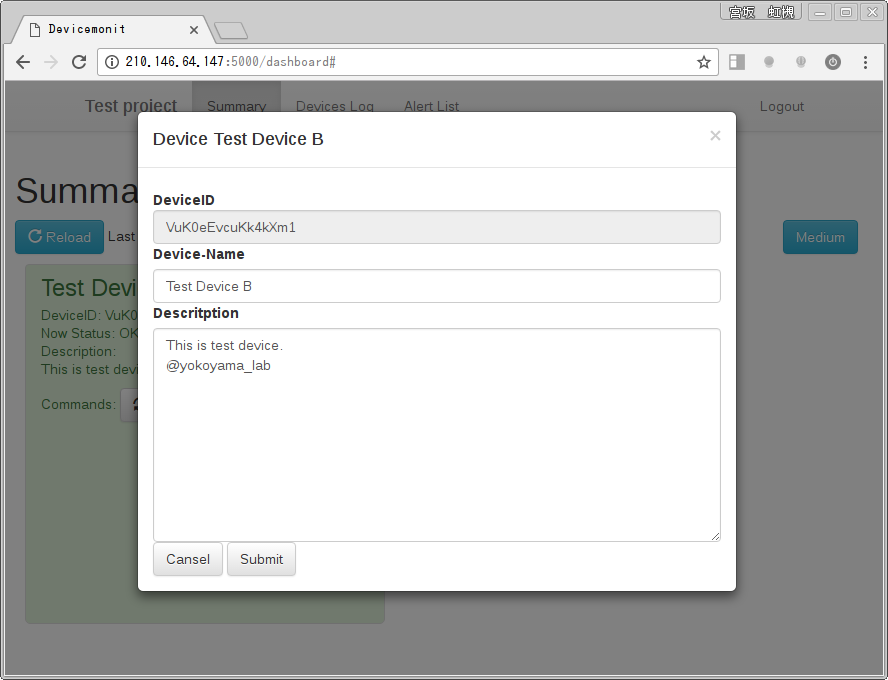
\includegraphics[width=16cm]{images/screenshot_mod.png}
		\caption{機器情報編集ダイアログ}
		\label{fig:ss_mod}
		\end{figure}


	\item 過去の機器状態一覧ページ\\
		過去の機器状態を時刻と共に整理し,一覧表示するページである.
		現在の機器の状態を取得するため,定期的にWebアプリケーションサーバと通信をする.
		図\ref{fig:ss_logs}は、スクリーンショットである。
		\begin{figure}[htbp]
		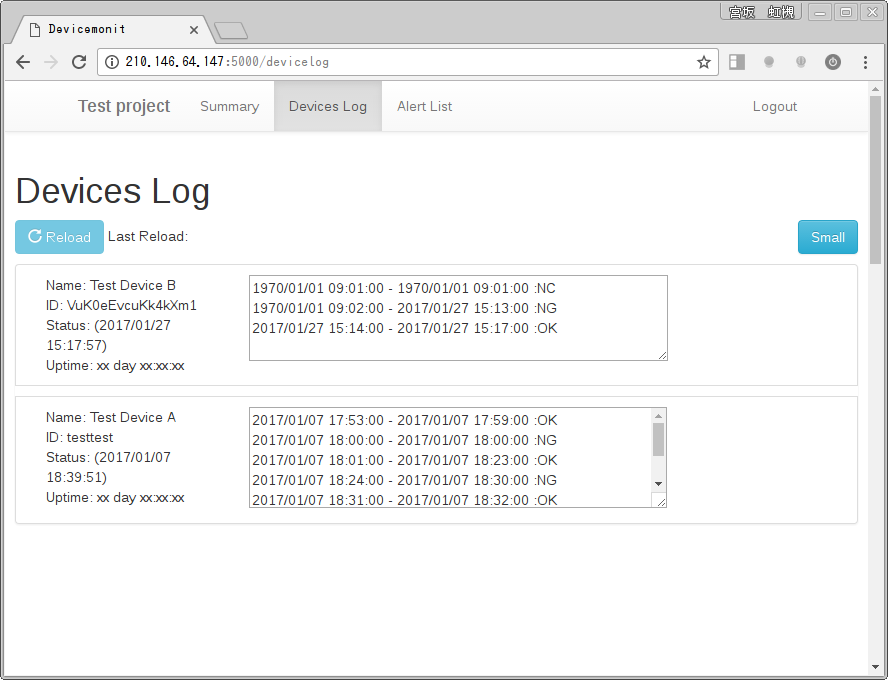
\includegraphics[width=16cm]{images/screenshot_logs.png}
		\caption{過去の状態表示ページ}
		\label{fig:ss_logs}
		\end{figure}

\end{itemize}

\section{エージェントプログラムの実装}
エージェントプログラムの役割は,送信失敗回数を定期的にIoT機器監視サーバーに送信することにある.
約1分おきに,現在の送信失敗回数と過去の送信失敗回数を,「かおりちゃん」へ送信する.
どのようなLinux環境でも動作することを考え,Shellスクリプトにて実装した.
\medskip

エージェントプログラムの動作は次のようになる.
\begin{enumerate}
\item エージェントプログラムが起動されると,まず過去に記録された送信失敗回数を読み出す.
\item 「かおりちゃん」に対し,過去に記録された送信失敗回数と,現在の送信失敗回数を送信する.%そうか!送信失敗回数は2種類ある!この説明をせねば!
\item サーバーから応答があった場合,過去に記録された送信失敗回数と,現在の送信失敗回数をクリアしする.\\
サーバーから応答がない場合,現在の送信失敗回数をインクリメントする.
\item 1分間スリープし,再び2から繰り返す.
\end{enumerate}


\section{エージェントプログラム用インターフェース「かおりちゃん」の実装}
「かおりちゃん」の役割は,エージェントプログラムから送信失敗回数を受け取り,時刻と正常である旨を機器状態データベースへ書き込むこと,
また,エージェントプログラムから送られた送信失敗回数から,インターネットより切断された時刻を逆算し,機器状態データベースへ書き込む事である.
Falconと呼ばれるAPIの作成に特化したフレームワークを使用し,Pythonにて実装した.
また,機器状態データベースへの書き込みには,InfluxDBClientというライブラリを使用した.

\section{機器情報データベース}
機器情報データベースの役割は,機器の名前,機器の詳細説明,機器ID,ユーザーID,ログイン用メールアドレスとパスワードを記録し保持する事である.
ユーザIDとは,システムにてユーザーを識別するための識別子である.
機器IDは,システムにてIoT機器識別するための識別子である.
機器情報データベースには,SQLitei3を用いた.
機器情報データベースには,次のようなテーブルが用意されている.
\subsection{機器情報テーブル}
機器ID,ユーザーIDをキーとして,機器の名前,機器の詳細説明を記録し保持するテーブルである.

\begin{comment}
\begin{table}[htb]
\begin{center}
\caption{}
\begin{tabular}{|l|l|l|} \hline
フィールド名 & 型 & 制約\\ \hline \hline
牛丼 & 並盛 & 500円 \\
牛丼 & 大盛 & 1,000円 \\
牛丼 & 特盛 & 1,500円 \\ \hline
牛皿 & 並盛 & 300円  \\
牛皿 & 大盛 & 700円 & 300 kcal \\
牛皿 & 特盛 & 1,000円 & 350 kcal \\ \hline
\end{tabular}
\label{tab:}
\end{center}
\end{table}
\end{comment}

\subsection{ユーザーテーブル}
ユーザーIDをキーとして,ユーザー名とパスワードを記録し保持するテーブルである.

\section{機器状態データベース}
機器状態データベースの役割は,機器の状態を時刻と共に記録・保持することである.
機器状態データベースには,Influxdbを用いた.
機器IDをメトリクス名(テーブル名)とし,時刻をキーとして,機器の状態を記録している.

\section{Webサーバーアプリケーション}
Webサーバーアプリケーションの役割は,与えられたHTTPリクエストを元に,Webページや,各種情報を返却することにある.
Flaskと呼ばれるWebアプリケーションフレームワークを用いた.Pythonを使用している.
Webサーバーアプリケーションの設計とWebアプリケーションの設計から,下記の様に実装した.
先頭に付いているGETやPOSTはHTTPメソッド,/login等はURLを示している.
\begin{description}
	\item[GET /login]\mbox{}\\
		ログインページを返す.
	\item[POST /login]\mbox{}\\
		メールアドレスとパスワードを受け取る.
		クッキーからセッションキーを探し,存在すれば既にログインしているとして,/dashboardへのリダイレクトメッセージを返す.
		データベースにメールアドレスとパスワードの組が存在するか確認し,存在した場合,セッションキーを返す.
		存在しなかった場合,ログインエラーページを返す.
	\item[GET /logout]\mbox{}\\
		セッションキーを受け取り,該当のセッションを削除する.
	\item[GET /dashboard]\mbox{}\\
		ログインチェックをし,機器状態一覧ページを返す.
	\item[GET /devicelog]\mbox{}\\
		ログインチェックをし,過去の機器状態一覧ページを返す.
	\item[GET /api/device/all]\mbox{}\\
		ログインチェックをし,現在の状態,最後にメッセージを受け取った日時,機器ID,機器名,機器詳細のデータを,JSON形式にまとめたものを返す.
	\item[GET /api/deviceID]\mbox{}\\
		ログインチェックをし,ランダムにデバイスIDを生成し,JSON形式にまとめたものを返す.
	\item[POST /api/deviceID]\mbox{}\\
		ログインチェックをし,受け取ったデバイスIDが既に存在するか確認し,その結果をJSON形式にまとめ,返す.
	\item[POST /api/device/\{DeviceID\}]\mbox{}\\
		ログインチェックをし,デバイスIDと受け取ったJSONデータから,デバイスの新規作成・編集をし,結果をJSON形式にまとめ,返す.
	\item[DELETE /api/device/\{DeviceID\}]\mbox{}\\
		ログインチェックをし,該当のデバイスIDを持つデバイスをデータベースから削除する.	
\end{description}


\section{Webアプリケーション}
Webアプリケーションの役割は,ユーザーインターフェースを提供することである.
Bootstrap,JQueryというライブラリを用いて作成した.HTML,CSS,Javascriptで書かれている.
定期的にWebアプリケーションサーバから状態を取得し,HTML,CSSを用いて表示する.

\section{エージェントプログラムと「かおりちゃん」間の通信の実装}
%このような形式で,どんな情報を伝えているのか.
%特徴としてどのような事があるのか
エージェントプログラムと「かおりちゃん」は,インターネットを介して,HTTPというプロトコルを用いて通信する.
エージェントプログラムと「かおりちゃん」間の通信は次の様な形になる.
\begin{enumerate}
	\item エージェントプログラムが「かおりちゃん」に対し,送信失敗回数を報告する.
	\item 「かおりちゃん」は,時刻と正常である旨を機器状態データベースへ送信する.
	\item 機器状態データベースより,正常に書き込んだというメッセージが帰ってくる.
	\item 「かおりちゃん」は,必要に応じて送信失敗回数からインターネットから切断された時刻を逆算し,その時刻と切断されていた旨を機器状態データベースへ送信する.
	\item 機器状態データベースより,正常に書き込んだというメッセージが帰ってくる.
	\item 「かおりちゃん」は,エージェントプログラムに対し,正常に受け付けたというメッセージを返す.
\end{enumerate}
エージェントプログラムと「かおりちゃん」の間の通信は,約1分おきに繰り返される.
\begin{figure}[htbp]
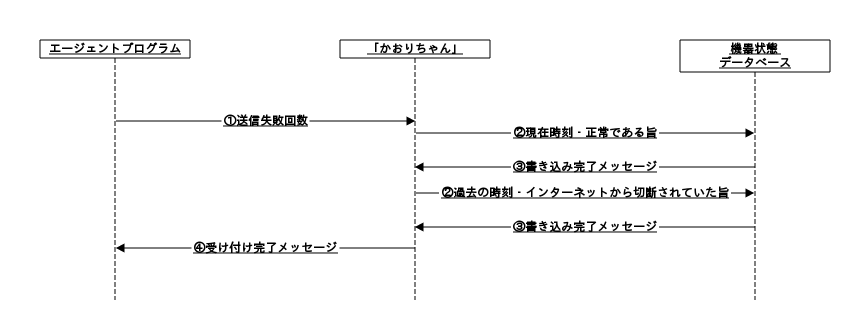
\includegraphics[width=16cm]{images/seq1.png}
\caption{エージェントプログラムと「かおりちゃん」の間のメッセージシーケンス図}
\label{fig:blockdiagram}
\end{figure}

HTTP上でやり取りするデータの形式としては,Javascript Object Notation(JSON)という形式を用いる.
エージェントプログラムからは,次のような形式でメッセージが送られる.
\begin{lstlisting}[caption=エージェントプログラムから「かおりちゃん」に送られるメッセージの書式,label=format1]
{"seq":<NOW>, "stat":"OK", "log":{"seq":<PAST>}}
\end{lstlisting}
<NOW> には,現在の送信失敗回数が入る.
<PAST> には,過去の送信失敗回数が入る.


また,「かおりちゃん」からは,次のような形式で応答がある.
\begin{lstlisting}[caption=「かおりちゃん」からエージェントプログラムへの応答の形式,label=format2]
{"stat":"OK", "time":<NOWTIME> }
\end{lstlisting}
ここで,<NOWTIME> にはサーバー側の現在時刻が入る.


\section{WebアプリケーションサーバとWebアプリケーション間の通信の実装}
%どのような形式で,どのような情報を伝えているのか.
WebアプリケーションサーバとWebアプリケーションは,インターネットを介し,HTTPというプロトコルを用いて通信する.
HTTP上でやり取りするデータの形式としては,Javascript Object Notation(JSON)という形式を用いる.

\section{サービスによる監視のイメージ}
%ユーザー目線で,ユーザーは何をしてこれこれこうする みたいな.
本サービスで想定するユーザーの動きをまとめる.
\begin{itemize}
\item ユーザーがIoT機器をサービスに登録する場合
	\begin{enumerate}
	\item ユーザーは最初にサービスにログインし,機器一覧ページへ遷移する.
	\item ユーザーは機器一覧ページにある「+」ボタンを押す.すると,機器追加用ダイアログが表示される.
	\item 機器IDが既に決まっている場合は,機器ID欄を書き換える.\\
		決まっていない場合は,機器ID欄に表示されている機器IDをメモしておく.
	\item 機器名,機器詳細を入力する.
	\item 機器の追加ボタンを押し,機器一覧に追加した機器が表示されていることを確認する.
	\item ユーザーは,IoT機器へエージェントプログラムをインストールし,自動でエージェントプログラムが起動するよう設定する.
	\item ユーザーは,IoT機器をインターネットに繋ぎ,サービスの機器状態一覧ページの表示が変わったことを確認する.
	\end{enumerate}
\item ユーザーがIoT機器の情報を変更する場合
	\begin{enumerate}
	\item ユーザーは,サービスにログインし,機器一覧ページへ遷移する.
	\item 該当の機器をクリックし開く.
	\item 該当の機器の編集ボタンを押すと,機器情報編集ダイアログが表示される.
	\item 機器名,機器詳細を編集し,OKボタンを押す.
	\end{enumerate}
\item ユーザーがIoT機器を削除する場合
	\begin{enumerate}
	\item ユーザーは,サービスにログインし,機器一覧ページへ遷移する.
	\item 該当の機器をクリックし開く.
	\item 該当の機器の削除ボタンを押すと,確認ダイアログが表示されるので,OKを押す.
	\item 機器一覧ページから,機器が消えたことを確認する.
	\end{enumerate}
\item ユーザーが現在の機器の情報,機器の状態を確認する場合
	\begin{enumerate}
	\item ユーザーはサービスにログインし,機器一覧ページへ遷移する.
	\item 該当の機器をクリックし開くと,機器の情報がと,現在の状態,最後に通信があった日時等が表示される.
	\item また,機器一覧ページにて機器の背景が,緑色である場合は正常で,赤色である場合は異常である.
	\end{enumerate}
\item ユーザーが過去の機器状態を確認する場合
	\begin{enumerate}
	\item ユーザーは,サービスにログインし,機器一覧ページへ遷移する.
	\item ナビバーから過去の機器状態ページへ遷移する.
	\item すると,機器と機器の過去の状態一覧が表示されるので,該当の機器を見つけ出し,確認する.
	\end{enumerate}
\end{itemize}




